\documentclass[10pt,a4paper]{article}
\usepackage[margin=20mm]{geometry}
\usepackage[T1]{fontenc}
\usepackage{lmodern}
\usepackage{graphicx}
\usepackage{booktabs}
\usepackage{amsmath}
\usepackage{microtype}
\usepackage{hyperref}
\usepackage{fancyhdr}
\hypersetup{colorlinks=true,linkcolor=black,urlcolor=blue}
\pagestyle{fancy}
\fancyhf{}
\fancyhead[L]{Newton \textbar\ Moving terrain benchmark}
\fancyhead[R]{Box, rover, and G1}
\fancyfoot[C]{\thepage}
\setlength{\headheight}{13pt}
\setlength{\parindent}{0pt}
\setlength{\parskip}{5pt}
\title{Moving Terrain MPM: Computation and Memory Scaling}
\author{Newton simulation benchmark}
\date{September 23, 2026}

\begin{document}
\maketitle

\section*{Motivation}
Simulating all the sand in a large environment increases both particle storage and the work of each physics step. We evaluate whether a fixed-size moving patch can keep this cost bounded while a dynamic object or robot moves through a larger terrain. The benchmark compares fixed MPM grids, sparse MPM grids, and the beta moving-patch implementation in three scenes: a box, a four-wheel rover, and a G1 humanoid. All scenes use two-way rigid-body--MPM coupling. All three methods share the beta scene and coupling loop; the benchmark changes terrain allocation and grid handling.

\begin{figure}[htbp]
\centering
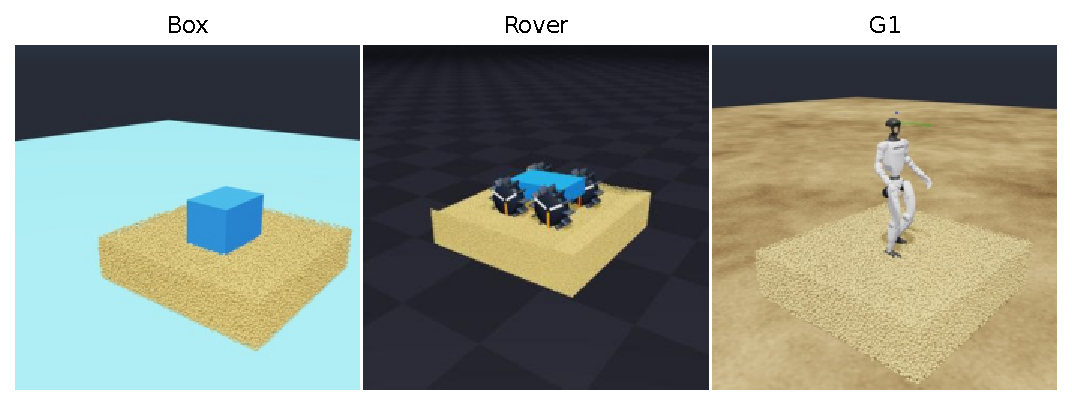
\includegraphics[width=\linewidth]{00_scenes.pdf}
\caption{The three example scenes. These existing viewer images identify the simulated objects; benchmark measurements run without rendering, with flat terrain and the common parameters in Table~\ref{tab:setup}.}
\end{figure}

\section{Methodology}
\subsection{Methods and terrain sizes}
\textbf{Fixed} uses the implicit MPM solver's fixed Cartesian grid, initialized around the particles with four voxels of padding. The solver still selects occupied cells for the material solve. \textbf{Sparse} uses a rebuildable sparse grid around particles. Its topology is stored in NanoVDB, a hierarchical voxel data structure, with a positive reserved active-cell capacity. \textbf{Moving-patch} uses the same sparse-grid configuration with \texttt{MovingTerrainMPMWrapper}. It retains particles inside the moving terrain and recycles particles that leave it. The beta height cache stores measured terrain height and reference material volume; it does not preserve full particle stress or deformation state.

For the scaling sweep, the listed terrain side length $L$ ranges from 3 to 10\,m in 1\,m increments. Fixed and sparse simulate an $L\times L\times0.5$\,m particle bed. Moving-patch always allocates a $3\times3\times0.5$\,m bed: a $2\times2$\,m area of simulated terrain surrounded by a 0.5\,m boundary on each side. Boundary particles remain active with zero mass, providing kinematic support. Fixed and sparse use the same boundary width at the edges of their full beds.

The background height map and supporting ground span $(L+2)\times(L+2)$\,m in every method. This adds travel margin around the particle bed, including the 3\,m case. The plotted $L$ describes the full particle bed for fixed and sparse, not the background map. Moving-patch background storage therefore grows with $L$, even though its MPM particle and grid allocation stays fixed. Height-update working arrays also keep the local patch dimensions.

For the overhead comparison, all three methods allocate identical particle beds with side lengths 1, 2, and 4\,m and depth 0.5\,m. Boundary width is 0.1\,m on each side for every method in this comparison, so the 1\,m case still has a nonzero area of simulated terrain. These cases isolate the practical cost of maintaining a moving patch at matched initial particle counts; subsequent particle positions and solver workloads can differ. The smallest bed places robot contacts close to the fixed terrain edge, so the 2\,m case is the main overhead reference.

\begin{table}[htbp]
\centering
\caption{Common benchmark settings.}\label{tab:setup}
\begin{tabular}{ll}
\toprule
Parameter & Value \\
\midrule
GPU & NVIDIA GeForce RTX 5090, approximately 32\,GiB \\
CPU & Intel Core Ultra 9 285K \\
Host memory visible to the OS & Approximately 62\,GiB \\
MPM voxel size & 0.05\,m \\
Particle sampling & 3 per axis per voxel; 27 per voxel \\
Particle spacing; jitter distance & $0.05/3$\,m; $0.05/3$\,m \\
Sand depth; density & 0.5\,m; 2500\,kg/m$^3$ \\
Young's modulus; Poisson ratio & 40\,MPa; 0.3 \\
Sand friction coefficient & $\tan(50^\circ)$ \\
Transfer; velocity/strain/collider bases & PIC; Q1 / P0 / S2 \\
Maximum MPM iterations; warm start & 50; automatic \\
Physics timestep & 0.005\,s (200\,Hz) \\
Controller frame rate; physics substeps & 50\,Hz; 4 \\
MuJoCo substeps per physics step & 4 \\
Proxy coupling passes; mass scale & 1; 1 \\
Commanded forward speed & 0.2\,m/s \\
Warm-up; measured steps per run & 150; 150 \\
Independent attempts per case & 2 \\
\bottomrule
\end{tabular}
\end{table}

Both sparse methods reserve at least 65,536 active cells. For a particle bed of width $W$, the capacity is
\[
 C=\max\left(65{,}536,\;22\left\lceil W/0.05+8\right\rceil^2\right).
\]
NanoVDB node capacities use the solver defaults. This tests the current conservative capacity policy, not a tuned minimum-memory sparse configuration or dynamic allocation with capacity $-1$. The same capacity rule is passed to fixed grids, although fixed-grid allocation follows its Cartesian bounds. Raw results record particle count, active-cell count, and capacity for each case.

\subsection{Motion, timing, and memory}
The box starts with its center at 0.8\,m, placing its bottom 0.05\,m above the sand, and follows a forward reference through a force controller. The rover uses differential-drive wheel commands. G1 runs its actuated policy at 50\,Hz with a forward velocity command. Bodies remain dynamic; prescribed commands do not overwrite their poses. The scenes use the same sampling and material settings, rather than their different interactive material presets.

Each case runs in a fresh process. We exclude initialization and 150 warm-up steps, then measure 150 individual physics steps with GPU synchronization after each step. Timing includes the scene controller, collision handling, two-way coupling, MPM solve, and moving-patch updates. G1 timing also includes policy inference when scheduled. Rendering, display compaction, and frame capture are excluded, and no outer CUDA graph is captured. Each run covers 1.5\,s of simulated time, of which the last 0.75\,s is measured. It measures a local forward segment, not traversal of the entire terrain.

Plots show the mean and sample standard deviation of successful measured steps pooled across the two attempted independent runs. Standard deviation describes step-time variation, not uncertainty in the estimated mean. Repeat order is reversed for the second sweep to reduce systematic ordering effects. Repeated runs, poses, particle recycling counts, and finite-state checks are retained in the raw data.

GPU memory is sampled through NVML at 20\,Hz, subtracting device usage before each process initializes CUDA. Plots show the mean and standard deviation of samples taken from the first measured step through the final state checks. The separately recorded sampled peak includes initialization. This measures the application's total GPU footprint, including solver storage, the CUDA context, robot assets, and G1 policy storage; it is not an isolated measurement of MPM arrays. GPU allocators may retain storage allocated during setup. Small memory differences can also include changes in desktop GPU usage because the measurement uses device-wide counters.

\section{Performance with fixed/sparse MPM grid}
Sparse allocation does not eliminate work on particles throughout a filled sand bed. Both full-terrain methods increase particle count from 972,000 at 3\,m to 10,800,000 at 10\,m. The following table compares the largest size completed by both methods for each scene. Times are mean $\pm$ standard deviation in milliseconds; memory is the measured mean in GiB.
\begin{center}\small\begin{tabular}{lrrrrr}\toprule
Scene & Side [m] & Fixed [ms] & Sparse [ms] & Fixed [GiB] & Sparse [GiB] \\\midrule
Box & 8 & $80.96\pm6.23$ & $186.86\pm2.68$ & 12.87 & 22.98 \\
Rover & 7 & $67.18\pm6.65$ & $148.46\pm3.17$ & 14.41 & 22.63 \\
G1 & 7 & $66.05\pm1.66$ & $142.98\pm2.39$ & 14.33 & 22.41 \\
\bottomrule\end{tabular}\end{center}
Sparse has a lower mean step time in 0 of 16 matched size/scene comparisons. These results describe the tested reserved-capacity configuration; they do not establish an inherent advantage for either grid representation. No component-level profiling was performed to separate grid rebuilding, material solving, and capacity-related costs.
5 attempts failed during GPU memory allocation with the tested settings.
4 initialization workers were terminated by SIGKILL before measurements; the cause could not be confirmed because kernel logs were not accessible.
Failed measurements are excluded from means and shown as missing plot points. The affected cases and failure messages are listed in the accompanying summary data.
Box sparse: failed runs at side lengths 10, 9\,m.
Rover fixed: failed runs at side lengths 10\,m.
Rover sparse: failed runs at side lengths 10, 8, 9\,m.
G1 fixed: failed runs at side lengths 10\,m.
G1 sparse: failed runs at side lengths 10, 8, 9\,m.

\begin{figure}[p]
\centering
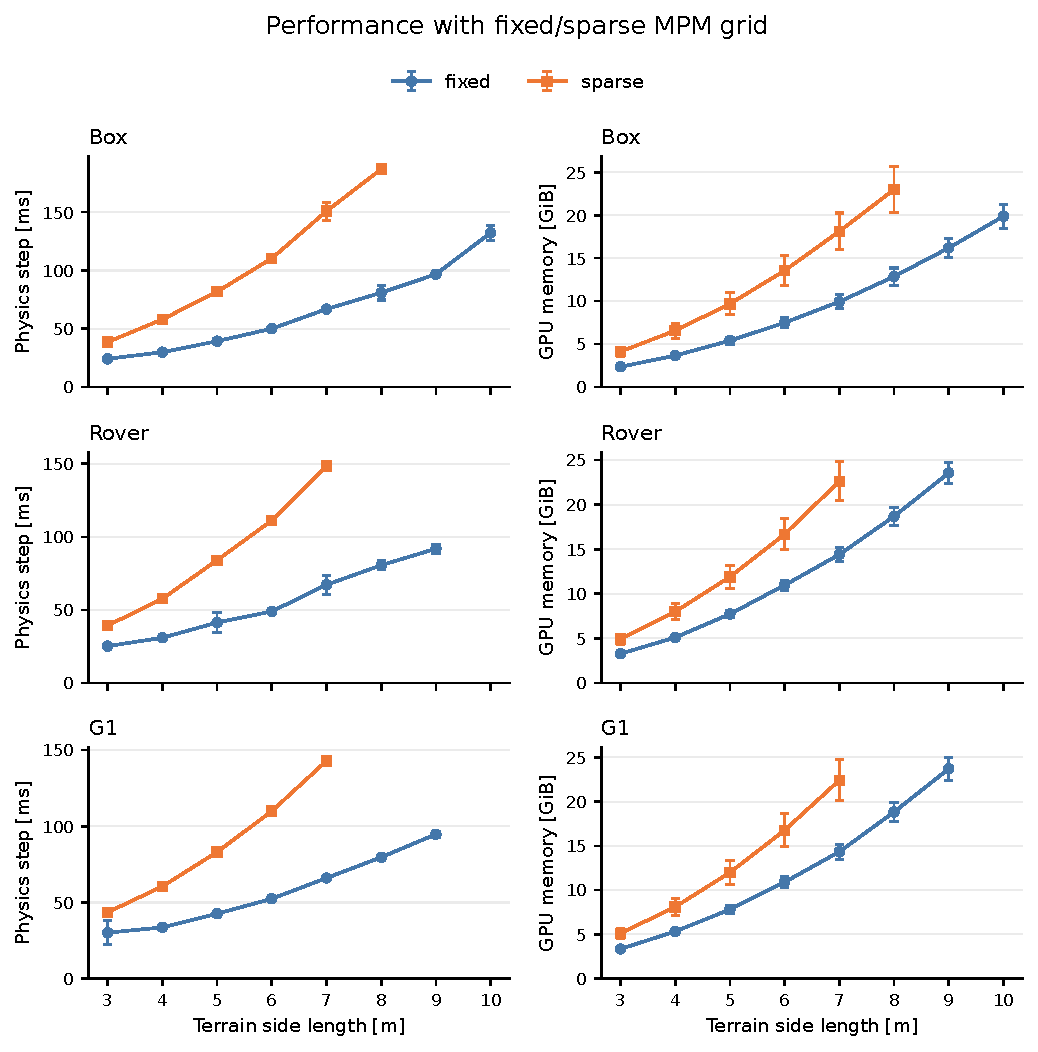
\includegraphics[width=\linewidth]{01_grid_comparison.pdf}
\caption{Fixed and sparse full-terrain simulations. Points show mean completed physics-step time and mean measured GPU memory; error bars show one sample standard deviation. Rows correspond to box, rover, and G1. Missing points indicate no successful repeat; failures are listed in the results.}
\end{figure}

\section{Terrain size scaling}
Moving-patch keeps 972,000 MPM particles for every background size in this sweep. The measured ranges across 3--10\,m are:
\textbf{Box:} 38.65--43.70\,ms per step and 4.11--4.20\,GiB mean GPU memory.
\textbf{Rover:} 38.63--43.96\,ms per step and 4.87--5.01\,GiB mean GPU memory.
\textbf{G1:} 42.18--42.38\,ms per step and 5.02--5.50\,GiB mean GPU memory.
At the 10\,m endpoint, the comparison is:
\begin{center}\small\begin{tabular}{llrr}\toprule
Scene & Method & Time [ms] & Memory [GiB] \\\midrule
Box & fixed & $132.30\pm6.61$ & $19.87\pm1.41$ \\
Box & sparse & --- & --- \\
Box & moving-patch & $43.70\pm1.76$ & $4.20\pm0.51$ \\
Rover & fixed & --- & --- \\
Rover & sparse & --- & --- \\
Rover & moving-patch & $39.37\pm1.36$ & $5.00\pm0.53$ \\
G1 & fixed & --- & --- \\
G1 & sparse & --- & --- \\
G1 & moving-patch & $42.19\pm1.83$ & $5.13\pm0.53$ \\
\bottomrule\end{tabular}\end{center}
The full-terrain methods retain all particles as terrain size grows. Moving-patch instead limits the local material simulation to a fixed allocation. Its background height map and ground still grow with terrain area, so approximately flat curves over this range do not imply constant memory for an arbitrarily large background.

\begin{figure}[p]
\centering
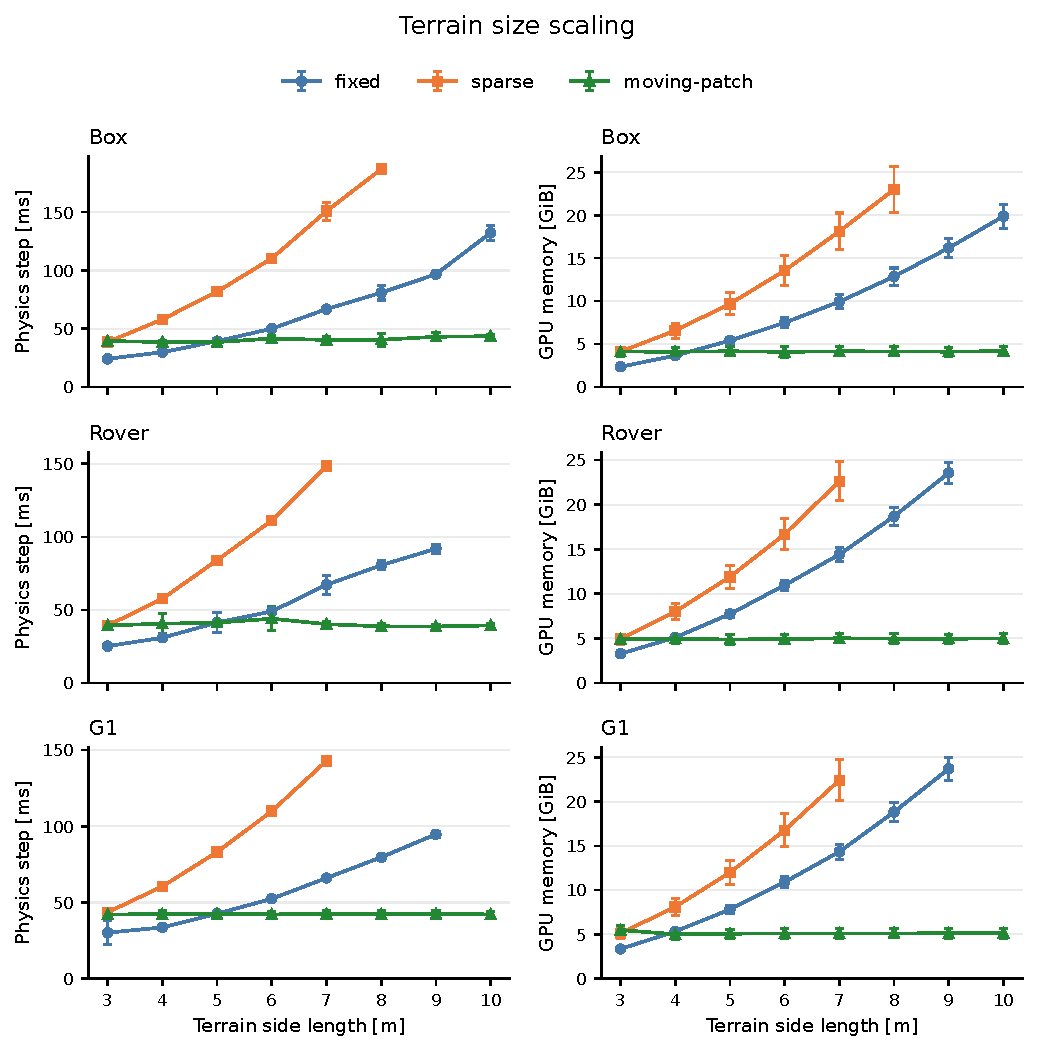
\includegraphics[width=\linewidth]{02_terrain_scaling.pdf}
\caption{Full-terrain fixed and sparse methods compared with a fixed-size moving patch. Every moving-patch point is measured independently with its corresponding background map. The MPM particle count stays fixed for moving-patch; background map and ground storage grow with the listed terrain size.}
\end{figure}

\section{Moving patch compute/memory overhead}
Matched allocations contain 108,000, 432,000, and 1,728,000 particles for 1, 2, and 4\,m side lengths, respectively. At the 2\,m allocation:
\begin{center}\small\begin{tabular}{llrr}\toprule
Scene & Method & Time [ms] & Memory [GiB] \\\midrule
Box & fixed & $28.89\pm19.42$ & $1.42\pm0.06$ \\
Box & sparse & $31.01\pm16.03$ & $2.72\pm0.33$ \\
Box & moving-patch & $33.09\pm15.70$ & $2.75\pm0.36$ \\
Rover & fixed & $24.33\pm1.23$ & $1.98\pm0.08$ \\
Rover & sparse & $30.74\pm1.24$ & $3.06\pm0.35$ \\
Rover & moving-patch & $30.96\pm1.11$ & $3.15\pm0.33$ \\
G1 & fixed & $26.26\pm1.46$ & $1.98\pm0.06$ \\
G1 & sparse & $33.21\pm1.43$ & $3.25\pm0.35$ \\
G1 & moving-patch & $33.52\pm1.64$ & $3.22\pm0.34$ \\
\bottomrule\end{tabular}\end{center}
For Box, moving-patch minus sparse is +2.08\,ms (+6.7\%) and +0.03\,GiB. Moving-patch minus fixed is +4.21\,ms and +1.33\,GiB.
For Rover, moving-patch minus sparse is +0.22\,ms (+0.7\%) and +0.09\,GiB. Moving-patch minus fixed is +6.63\,ms and +1.17\,GiB.
For G1, moving-patch minus sparse is +0.31\,ms (+0.9\%) and -0.03\,GiB. Moving-patch minus fixed is +7.26\,ms and +1.24\,GiB.
The sparse comparison is the closer estimate of moving-patch overhead because it keeps the same grid representation. Differences against fixed include both grid implementation and moving-patch handling. The measurements include height-cache updates and particle recycling, but do not isolate those kernels; differences should not be attributed entirely to recycling.

\begin{figure}[p]
\centering
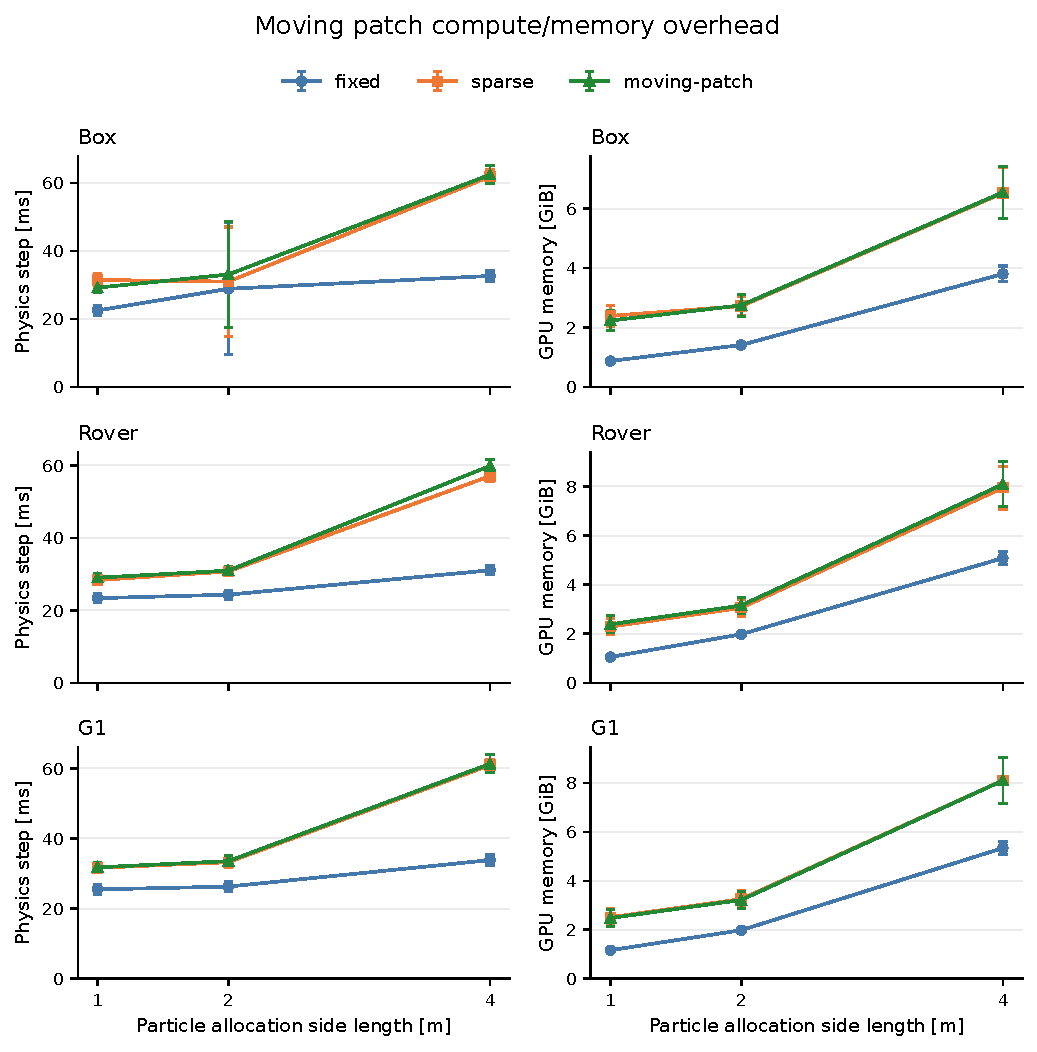
\includegraphics[width=\linewidth]{03_equal_size_comparison.pdf}
\caption{Matched initial particle allocations. All methods use the same 0.1\,m boundary width. Differences include moving-patch maintenance, terrain-history storage, and the resulting differences in the subsequent simulation workload. Error bars show one sample standard deviation.}
\end{figure}

\clearpage
\section{Scope and reproducibility}
These measurements evaluate performance with one dynamic object or robot on flat homogeneous terrain. They do not establish long-distance stability, accuracy of restored terrain deformation, standing stability, or scaling to many robots. Equal commands do not guarantee identical trajectories after terrain recycling. Sparse performance also depends on material occupancy and reserved grid capacity; results for these filled rectangular beds should not be generalized to disconnected or highly irregular material distributions.

The moving patch bounds local MPM work, but finite background storage remains proportional to the map area. A larger scene would eventually require a different background-storage policy. Measurements therefore support bounded local simulation cost over the tested sizes, rather than unlimited terrain storage at constant memory.

The benchmark directory contains \texttt{run\_benchmarks.py}, \texttt{plot\_results.py}, per-run JSON and logs in \texttt{raw/}, and aggregated \texttt{summary.csv} and \texttt{summary.json}. Hardware, software versions, source and asset hashes, and GPU process activity are stored alongside them. \texttt{README.md} gives the exact run and plot commands. No LaTeX compiler was installed in the measurement environment; this report is supplied as source with vector PDF and PNG figures.

\end{document}
